\begin{frame}{Model}
    \framesubtitle{General form}
        For \( u(x,t) \)
        \begin{equation}
        \text{ s.t. } u_t + \mathcal{N}[u] = 0
        \end{equation}
        Define  
        \begin{equation}
        f := u_t + \mathcal{N}[u]
        \end{equation}
        Then the minimize problem is:
        \begin{equation}
        \min\limits_{u} \text{MSE} = \text{MSE}_u + \text{MSE}_f
        \end{equation}
        where
        \begin{equation}
        \text{MSE}_u = \frac{1}{N_u} \sum_{i=1}^{N_u} | u(t_i^u, x_i^u) - u_i |^2
        \end{equation}
        \begin{equation}
        \text{MSE}_f = \frac{1}{N_f} \sum_{i=1}^{N_f} | f(t_i^f, x_i^f) |^2
        \end{equation}
    \end{frame}
    
    \begin{frame}{Model}
        \begin{block}{Penalty term}
        When we refer to LASSO, the MSE term includes two parts:\\
        the residual and the penalty (which is \( L_1 \) norm of the parameter).\\
        Now, it's actually setting the penalty term as:\\
        \begin{center}
        how far \( f \) is away from 0\\
        \end{center}
        with the physics constraint: 
        \begin{equation}
        f := u_t + \mathcal{N}[u]=0
        \end{equation}
        \end{block}
    \end{frame}
    
    \begin{frame}{Model}
    \framesubtitle{Discrete form and Runge-Kutta method}
        \begin{block}{Runge-Kutta method (Example of a 4-step RK)}
        Rewrite \( u_t + \mathcal{N}[u] = 0 \) in the form \( u_t = -\mathcal{N}[u] \).\\
        Start with \( u(0, x) = u_0(x) \):
        \begin{enumerate}
            \item Calculate the intermediate values \( k_1, k_2, k_3, k_4 \):
            \begin{align*}
                k_1 &= -\tau \mathcal{N}[u_n], \\
                k_2 &= -\tau \mathcal{N} \left( u_n + \frac{1}{2} k_1 \right), \\
                k_3 &= -\tau \mathcal{N} \left( u_n + \frac{1}{2} k_2 \right), \\
                k_4 &= -\tau \mathcal{N} \left( u_n + k_3 \right).
            \end{align*}
    
            \item Update the solution \( u \) at the next time step:
            \[
            u_{n+1} = u_n + \frac{1}{6} (k_1 + 2k_2 + 2k_3 + k_4).
            \]
        \end{enumerate}
        \end{block}
    \end{frame}
    
    \begin{frame}{Model}
    \framesubtitle{Discrete form and Runge-Kutta method}
        Apply the q-step Runge-Kutta to the general form to create the discrete estimator:
        \begin{equation}
        u_{n+c_i} = u_n - \tau \sum_{j=1}^q a_{ij} \mathcal{N}[u_{n+c_j}], \quad i = 1, \ldots, q
        \end{equation}
        \begin{equation}
        u_{n+1} = u_n - \tau \sum_{j=1}^q b_j \mathcal{N}[u_{n+c_j}]
        \end{equation}
        And the SSE is:
        \begin{equation}
        \text{SSE}_n = \sum_{j=1}^{q+1} \sum_{i=1}^{N_n} \left| u_{n,j}(x_{n,i}) - u_{n,i} \right|^2
        \end{equation}
    \end{frame}    
    
    \begin{frame}{Model}
    \framesubtitle{With boundary on function \( u \) (or multiple equations)}
        The solution of a PDE could change significantly if the equation includes high-order terms.\\
        We may need to add boundary conditions on \( u \) and add another penalty term to the MSE function. That is:
        \begin{equation}
        \mathcal{B}(u) = 0
        \end{equation}
        \begin{equation}
        \text{MSE} = \text{MSE}_u + \text{MSE}_f + \text{MSE}_b
        \end{equation}
        where\\
        \( \mathcal{B}[\cdot] \) is a boundary operator corresponding to Dirichlet, Neumann, Robin, or periodic boundary conditions. 
        \begin{equation}
        \text{MSE}_b = \frac{1}{N_b} \sum_{i=1}^{N_b} | \mathcal{B}(u)(t_i^b, x_i^b) |^2
        \end{equation}
        We could also apply the rule to any other \( u \)-equations.
    \end{frame}
    
    \begin{frame}{Model}
    \framesubtitle{With weight on error}
        The error terms are not necessarily equally weighted.\\
        Given by Raissi, M., Perdikaris, P., Karniadakis, G. E. (2024).\\
        \textit{An Expert’s Guide to Training Physics-informed Neural Networks.}\\
        We could rewrite the MSE function as:
        \begin{equation}
        \text{MSE} = \lambda_u \text{MSE}_u + \lambda_f \text{MSE}_f + \lambda_b \text{MSE}_b
        \end{equation}
    \end{frame}
    
    \begin{frame}{Model}
    \framesubtitle{With weight on error}
        And the \( \lambda \)'s are estimated by:
        \begin{equation}
        \hat{\lambda}_u = \frac{\| \nabla_{\theta} \text{MSE}_u (\theta) \| + \| \nabla_{\theta} \text{MSE}_b (\theta) \| + \| \nabla_{\theta} \text{MSE}_f (\theta) \|}{\| \nabla_{\theta} \text{MSE}_u (\theta) \|}
        \end{equation}
        \begin{equation}
        \hat{\lambda}_f = \frac{\| \nabla_{\theta} \text{MSE}_f (\theta) \| + \| \nabla_{\theta} \text{MSE}_u (\theta) \| + \| \nabla_{\theta} \text{MSE}_b (\theta) \|}{\| \nabla_{\theta} \text{MSE}_f (\theta) \|}
        \end{equation}
        \begin{equation}
        \hat{\lambda}_b = \frac{\| \nabla_{\theta} \text{MSE}_b (\theta) \| + \| \nabla_{\theta} \text{MSE}_f (\theta) \| + \| \nabla_{\theta} \text{MSE}_u (\theta) \|}{\| \nabla_{\theta} \text{MSE}_b (\theta) \|}
        \end{equation}
        where \( \theta \) is the parameter of the network (weights and biases).
    \end{frame}
    
    \begin{frame}{Model}
    \framesubtitle{Estimated result}
        In the Neural Network, we solve the minimize problem of MSE on all potential functions \( u \).\\
        There are two typical ways of using the estimated result.
        \begin{enumerate}
            \item When we do not need the formula of \( u \):\\
            Sometimes we only need the point estimate of the function. It could be either because the analytical solution is hard to solve in a simple form, or because the point estimate is sufficient.
            
            \item When we need the formula of \( u \):
            We should follow the steps to solve for an analytical solution of \( u \):
            \begin{enumerate}
                \item Solve the PDE with function parameters remaining \( u(\gamma) \).
                \item Set an appropriate activation function.
                \item Fit the model to get the estimated \( \hat{u} \).
                \item Estimate the function parameter \( \gamma \) with \( \hat{u} \).
            \end{enumerate}
        \end{enumerate}
    \end{frame}
    
    \begin{frame}{Model}
    \framesubtitle{Prediction failed}
        There are some cases where the prediction may fail:
        \begin{enumerate}
        \item Local minimum.
        \item Convergence difficulty.
        \item Chaotic system.
        \item Physics constraint.   
        \end{enumerate}
        I will list examples for the third and fourth problems.
    \end{frame}
    
    \begin{frame}{Model}
    \framesubtitle{Chaotic system}
        The paper: Steger, S., Rohrhofer, F. M., Geiger, B. C. (2022).\\
        \textit{How PINNs cheat: Predicting chaotic motion of a double pendulum.}\\
        OpenReview shows the predicted result of a double pendulum movement.
        From the graph we could see, for different given conditions at \( t_0 \), the result could be extremely well-fitted or totally unreliable.
        \begin{figure}[H]
            \centering
            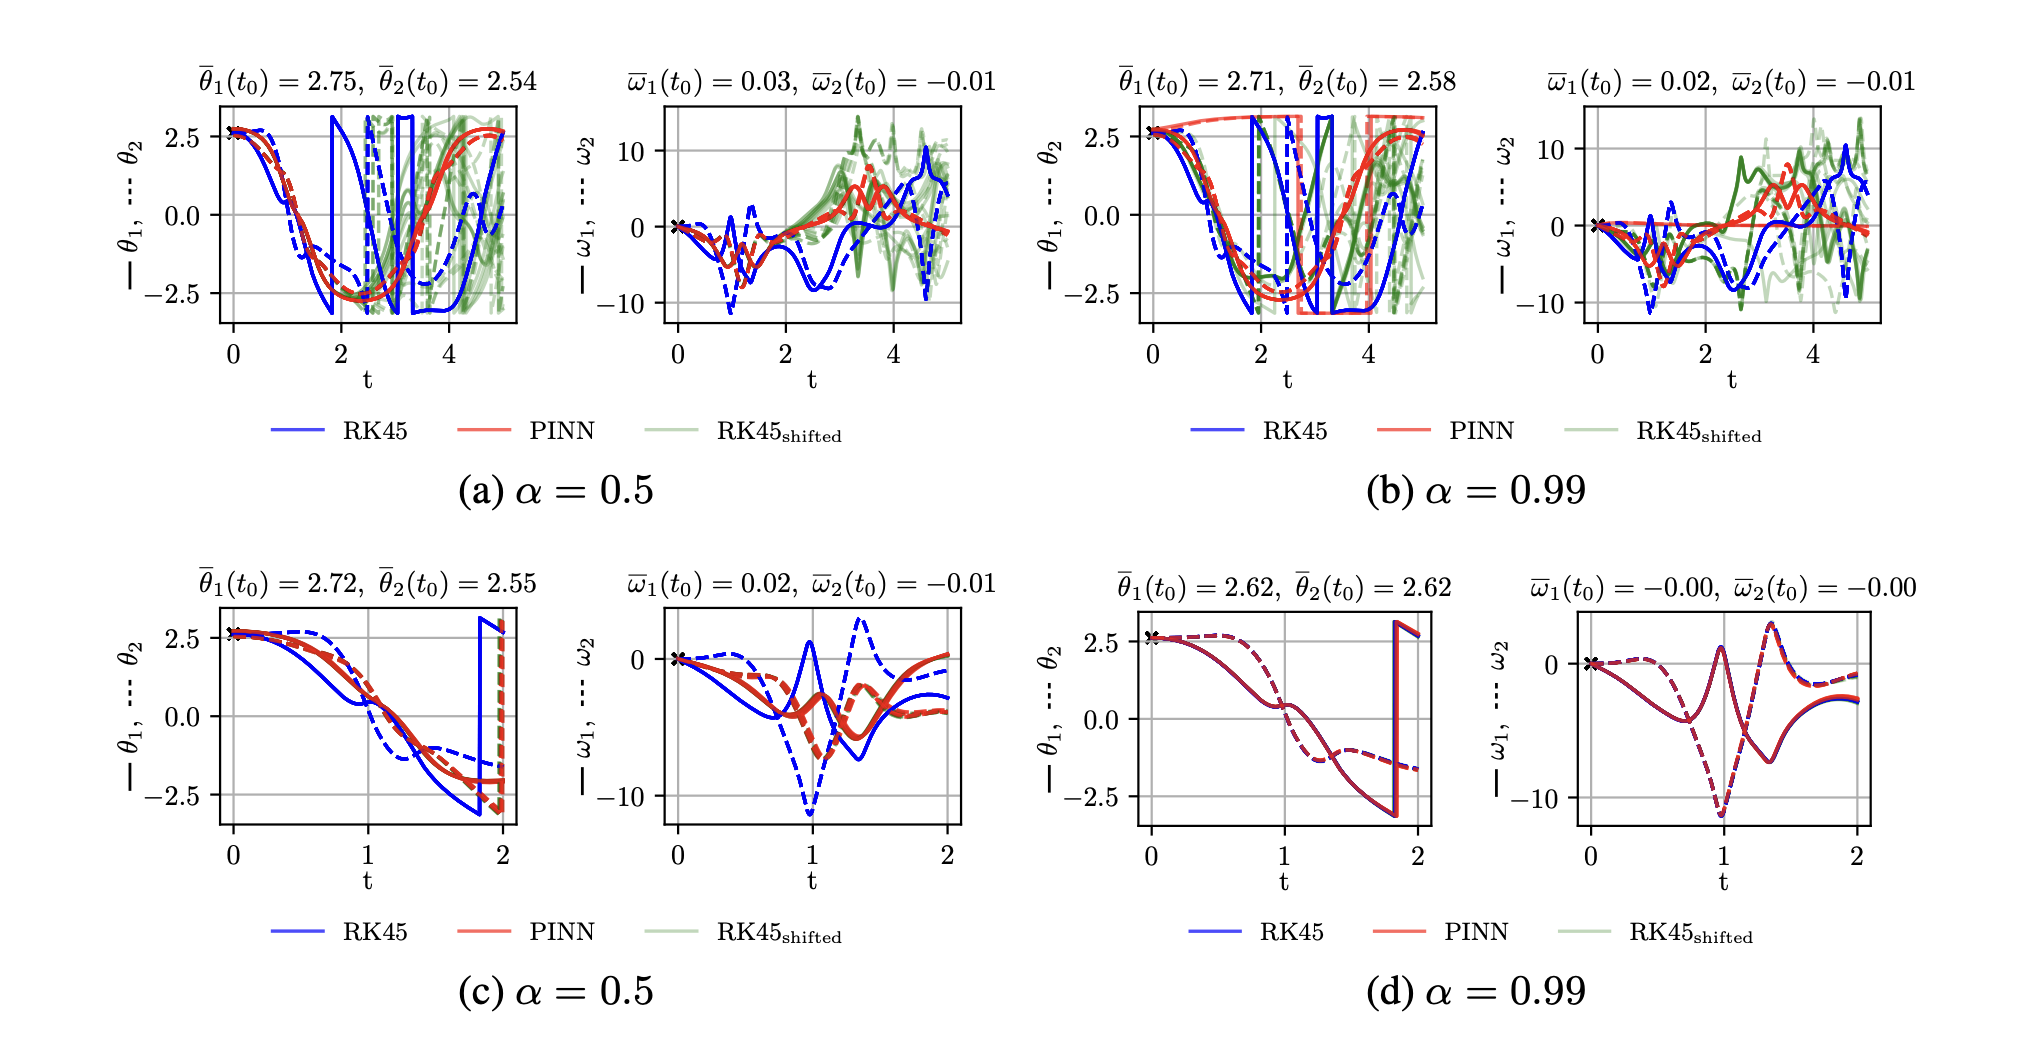
\includegraphics[width=0.8\textwidth]{img/Screenshot 2024-06-02 at 4.02.10 PM}
        \end{figure} 
    \end{frame}
    
    \begin{frame}{Model}
    \framesubtitle{Violate physical causality}
        The paper: Wang, S., Yu, X., Perdikaris, P. (2022).\\
        \textit{Respecting causality is all you need for training physics-informed neural networks.}\\
    
        In the paper, they discovered a convergence difficulty for the problem:
        \begin{equation}
        u_t - 0.0001u_{xx} + 5u^3 - 5u = 0, \quad t \in [0, 1], \quad x \in [-1, 1]
        \end{equation}
        \begin{equation}
        u(x, 0) = x^2 \cos(\pi x)
        \end{equation}
        \begin{equation}
        u(t, -1) = u(t, 1)
        \end{equation}
        \begin{equation}
        u_x(t, -1) = u_x(t, 1)
        \end{equation}
    \end{frame}
    
    \begin{frame}{Model}
    \framesubtitle{Violate physical causality}
        They then found out that because the residual is fitted on each time spot, it cannot capture the temporal causal relationships between physical variables. They adjusted the loss function by adding a weight with a causality parameter:
        \begin{equation}
        \mathcal{L}_r(\theta) = \frac{1}{N_t} \sum_{i=1}^{N_t} w_i \mathcal{L}_r(t_i, \theta)
        \end{equation}
        where
        \begin{equation}
        w_i = \exp \left( -\epsilon \sum_{k=1}^{i-1} \mathcal{L}_r(t_k, \theta) \right)
        \end{equation}
        and \( \epsilon \) is the causality parameter.
    \end{frame}
    
    \begin{frame}{Model}
    \framesubtitle{Violate physical causality: fitting result}
        \begin{figure}[H]
            \centering
            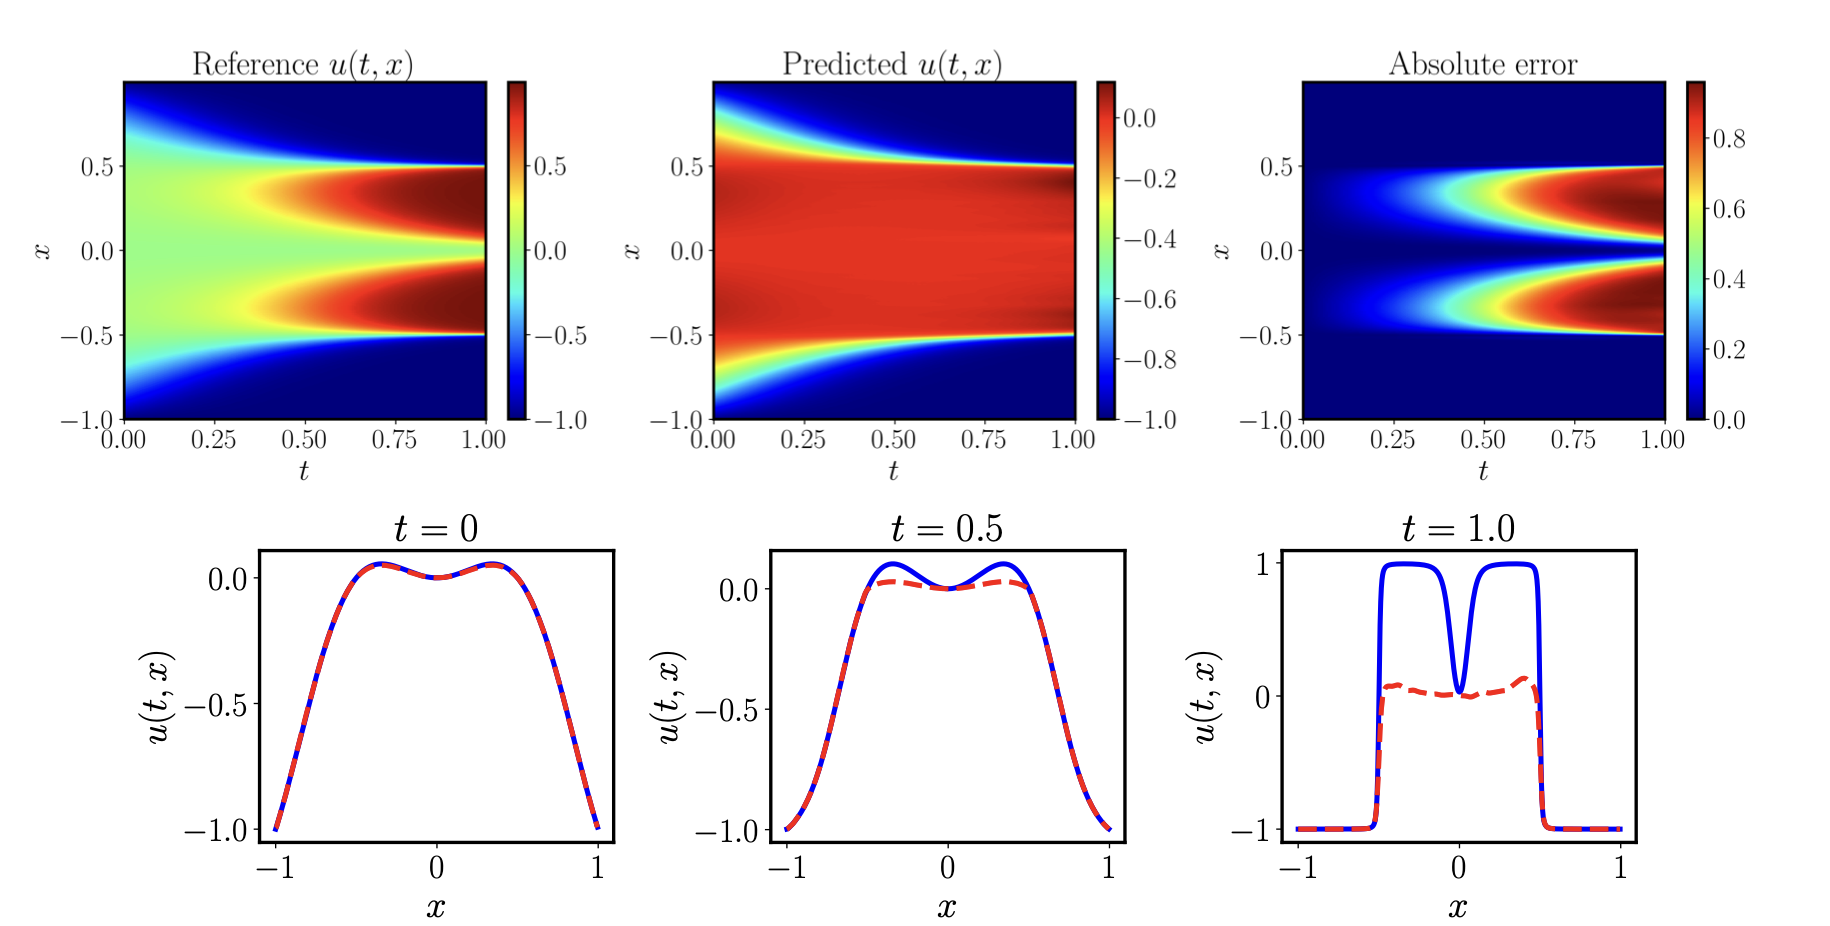
\includegraphics[width=0.55\textwidth]{img/Screenshot 2024-06-02 at 5.03.05 PM}
        \end{figure} 
        \begin{figure}[H]
            \centering
            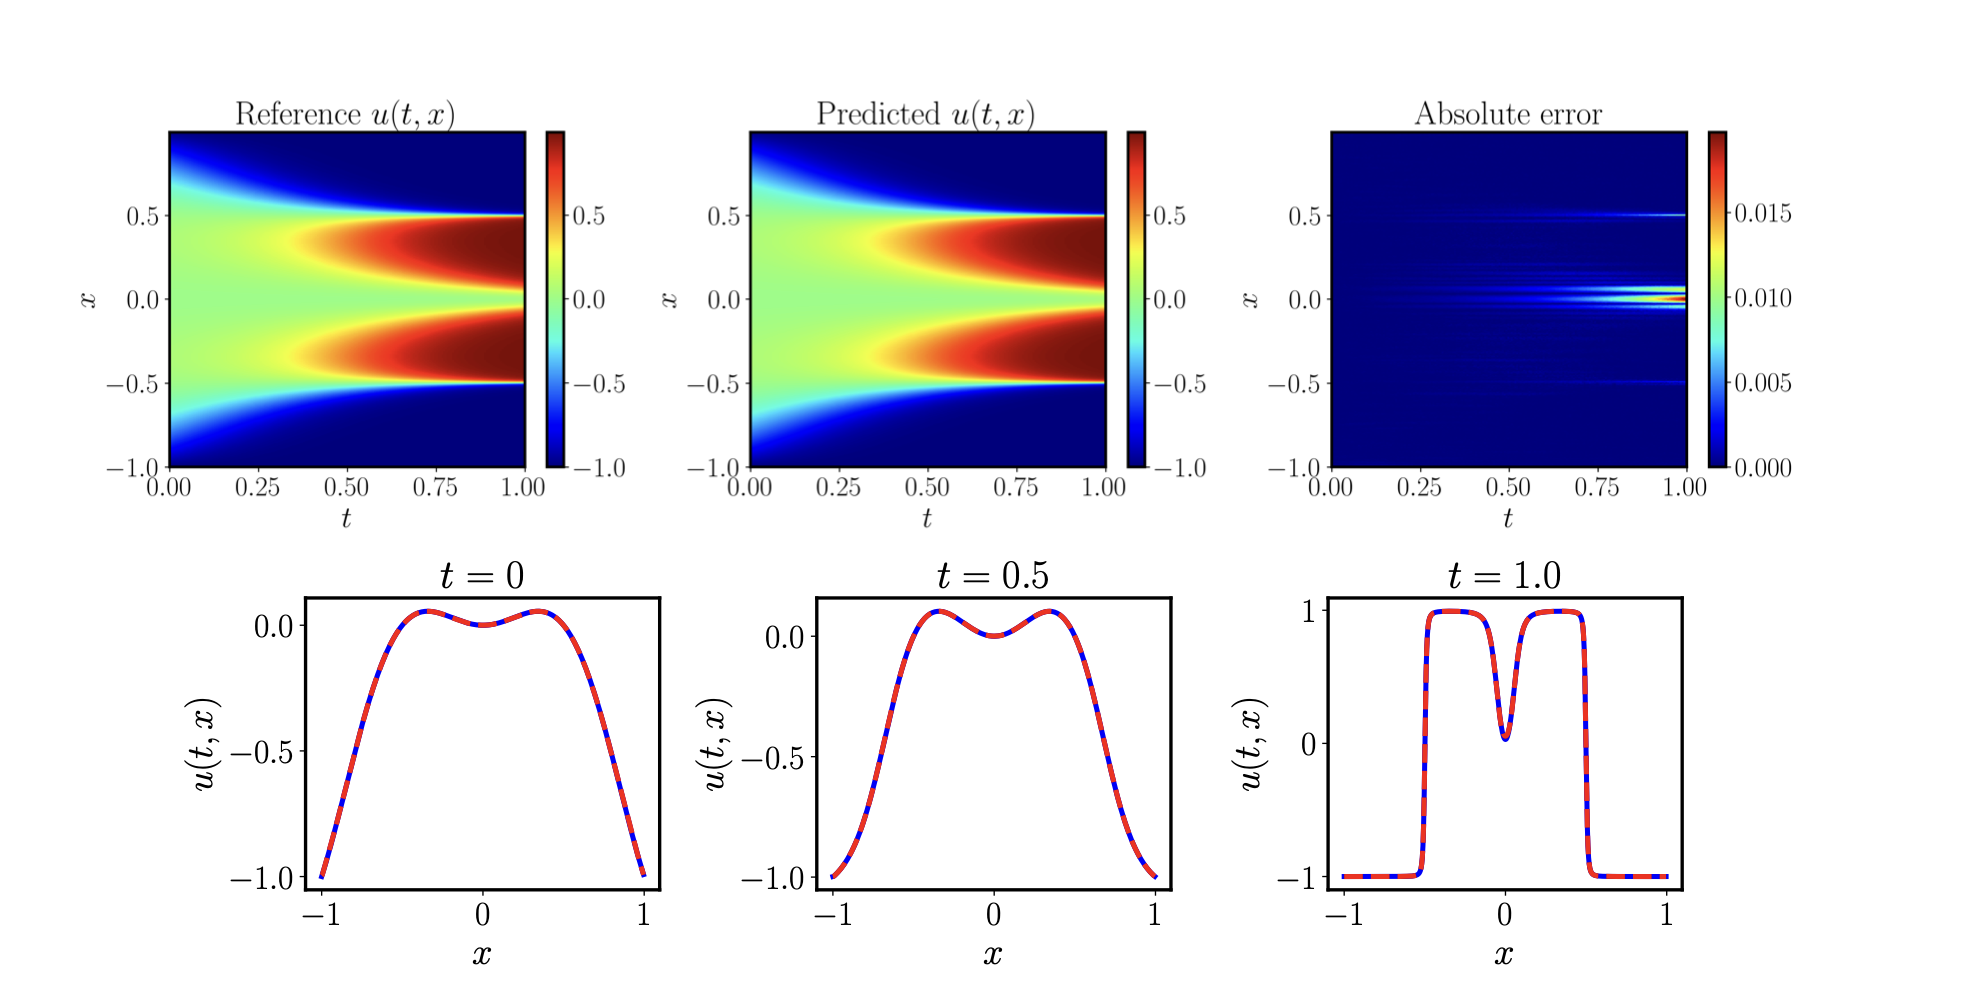
\includegraphics[width=0.6\textwidth]{img/Screenshot 2024-06-02 at 5.03.17 PM}
        \end{figure} 
    \end{frame}